\documentclass[a4paper,man,natbib]{apa6}

%%%%%%%%%%%%%%%%%%%%%%%%%%
% Thesis-specific settings
%%%%%%%%%%%%%%%%%%%%%%%%%%

%% BUG: title cannot be too long
\newcommand{\ThesisTitle}{KNOWLEDGE-DRIVEN AUDIO SCENE RECOGNITION}
\newcommand{\CThesisTitle}{����֪ʶ�����Ƶ����ʶ��}


%%%%%%%%%%%%%%%%
% Theme settings
%%%%%%%%%%%%%%%%

\usepackage{times}
%\linespread{1.5}

%\usepackage[a4paper,top=1.4in,head=1.5cm,headsep=0.5cm,bottom=1.28in,left=1.25in,right=1.25in]{geometry}

\usepackage{graphicx}
\usepackage{epstopdf}

%PURE's ADD
\usepackage{epsfig}
\usepackage{subfigure}
%\usepackage{indentfirst}
\usepackage{url}
\usepackage{array}
%END PURE's ADD

%\usepackage{fancyhdr}
%\fancypagestyle{plain}{%
%  \lhead{\includegraphics[width=4.3cm]{sjtubannerred}}
%  \chead{}
%  \rhead{\begin{minipage}{10cm}\begin{flushright}\fontsize{10pt}{12pt}\selectfont\ThesisTitle\end{flushright}\end{minipage}}
%  \lfoot{}
%  \cfoot{\fontsize{9pt}{9pt}\selectfont\thepage}
%  \rfoot{}
%  \renewcommand{\headrulewidth}{1pt}
%  \renewcommand{\footrulewidth}{0pt}}
%\pagestyle{plain}

%\title{\fontsize{16pt}{22pt}\selectfont\bf\ThesisTitle}
\title{Spatial Features in Classification of Geographic Points of Interest}
\shorttitle{Spatial Features in Classification of Geographic Points of Interest}
\fourauthors{Youer Pu}{Kaiqi Zhao}{Kenny Q. Zhu}{Gao Cong}
\fouraffiliations{Department of Computer Science \& Engineering\\ Shanghai Jiao Tong University\\ Shanghai, China}{School of Computer Engineering\\ Nanyang Technological University\\ Singapore}{Department of Computer Science \& Engineering\\ Shanghai Jiao Tong University\\ Shanghai, China}{School of Computer Engineering \\ Nanyang Technological University\\ Singapore}

%\usepackage{abstract}
%\renewcommand{\abstractname}{ABSTRACT}
%\renewcommand{\abstractnamefont}{\fontsize{14pt}{14pt}\selectfont\bf}
%\renewcommand{\abstracttextfont}{\fontsize{12pt}{16pt}\selectfont}
%\setlength{\absleftindent}{0pt}
%\setlength{\absrightindent}{0pt}

%\newcommand{\keywords}[1]{\noindent\textbf{Keywords:} #1}

%\usepackage[pdfborder=0 0 0,linktocpage=true]{hyperref}
%\usepackage{setspace}

%\usepackage{titlesec}
%\titleformat{\chapter}[block]{\fontsize{14pt}{14pt}\selectfont\centering\bf}{\chaptertitlename\ \thechapter}{14pt}{}{}
%\titleformat{\section}[block]{\fontsize{14pt}{14pt}\selectfont\bf}{\thetitle}{14pt}{}{}
%\titleformat{\subsection}[block]{\fontsize{14pt}{14pt}\selectfont\bf}{\thetitle}{14pt}{}{}
%\titleformat{\subsubsection}[block]{\fontsize{14pt}{14pt}\selectfont\bf}{\thetitle}{14pt}{}{}
%\titlespacing*{\chapter}{0pt}{0pt}{28pt}
%\titlespacing*{\section}{0pt}{16pt}{14pt}
%\titlespacing*{\subsection}{0pt}{16pt}{14pt}
%\titlespacing*{\subsubsection}{0pt}{16pt}{14pt}

%\usepackage[format=plain,labelsep=quad,font=bf]{caption}

%\usepackage[round,semicolon,authoryear,sort&compress]{natbib}
%\usepackage{apacite}
%\usepackage{natbib}
%\bibliographystyle{GBT7714-2005N}
%\bibliographystyle{apacite}
%\usepackage{apalike}
%\bibliographystyle{apalike}
\usepackage{apacite}
\bibliographystyle{apacite}

% add references to TOC
%\usepackage[nottoc]{tocbibind}
%\settocbibname{References}

% citation format: ([n], Author, Year: Page.)
%\let\oldcite\cite
%\usepackage{ifthen} % provides \ifthenelse test
%\usepackage{xifthen} % provides \isempty test
%\renewcommand{\cite}[2][]{%
%  \ifthenelse{\isempty{#1}}
%    {\oldcite{#2}}
%    {\citetext{[\citenum{#2}], \citeauthor{#2}, \citeyear{#2}: #1.}}}

\usepackage{amsmath,amssymb,amsthm}
%\makeatletter
%\long\def\theequation{\ifnum \c@chapter > \z@ \thechapter -\fi \@arabic \c@equation}
%\makeatother
%\newtheorem{theorem}[theorem][Theorem]
%\newtheorem{definition}[theorem]{Definition}
%\newtheorem{problem}[theorem]{Problem}
%\newtheorem{algorithm}[theorem]{Algorithm}
%\newtheorem{example}[theorem]{Example}

\usepackage{algpseudocode}
%\newcommand{\To}{\ \textbf{to}\ }

%\usepackage{tikz}
%\usetikzlibrary{matrix,positioning,fit,backgrounds}

%\newcommand{\eqn}[1]{Equation (\ref{eqn:#1})}
%\newcommand{\fig}[1]{Figure \ref{fig:#1}}

%\newcommand{\KQ}[1]{\textcolor{red}{[KQ: #1]}}
\usepackage[normalem]{ulem}
\usepackage{listings}
\usepackage{color}

%\definecolor{mygreen}{rgb}{0,0.6,0}
%\definecolor{mygray}{rgb}{0.5,0.5,0.5}
%\definecolor{mymauve}{rgb}{0.58,0,0.82}

%\lstset{ %
%  backgroundcolor=\color{white},   % choose the background color; you must add \usepackage{color} or \usepackage{xcolor}
%  basicstyle=\footnotesize\tt,     % the size of the fonts that are used for the code
%  breakatwhitespace=false,         % sets if automatic breaks should only happen at whitespace
%  breaklines=true,                 % sets automatic line breaking
%  captionpos=b,                    % sets the caption-position to bottom
%  commentstyle=\color{mygreen},    % comment style
%  deletekeywords={...},            % if you want to delete keywords from the given language
%  escapeinside={\%*}{*)},          % if you want to add LaTeX within your code
%  extendedchars=true,              % lets you use non-ASCII characters; for 8-bits encodings only, does not work with UTF-8
%  frame=single,                    % adds a frame around the code
%  keepspaces=true,                 % keeps spaces in text, useful for keeping indentation of code (possibly needs columns=flexible)
%  keywordstyle=\color{blue},       % keyword style
%  morekeywords={*,...},            % if you want to add more keywords to the set
%  numbers=left,                    % where to put the line-numbers; possible values are (none, left, right)
%  numbersep=9pt,                   % how far the line-numbers are from the code
%  numberstyle=\tiny\color{mygray}, % the style that is used for the line-numbers
%  rulecolor=\color{black},         % if not set, the frame-color may be changed on line-breaks within not-black text (e.g. comments (green here))
%  showspaces=false,                % show spaces everywhere adding particular underscores; it overrides 'showstringspaces'
%  showstringspaces=false,          % underline spaces within strings only
%  showtabs=false,                  % show tabs within strings adding particular underscores
%  stepnumber=1,                    % the step between two line-numbers. If it's 1, each line will be numbered
%  stringstyle=\color{mymauve},     % string literal style
%  tabsize=2,                       % sets default tabsize to 2 spaces
%  title=\lstname                   % show the filename of files included with \lstinputlisting; also try caption instead of title
%}

%%%%%%%%%%%%%%%%%%%%%%
% Document starts here
%%%%%%%%%%%%%%%%%%%%%%

\abstract{
The category of a point-of-interest (POI) is 
important for location based services (LBS). Popular map services try to
include POI type information or allow map users to tag POIs from a 
predefined set of categories, but these tags can be inaccurate and far from complete.
The classification of POIs have been studied in the context of location-based
social network and models are largely based on user visiting behaviors.
This paper explores another aspect of a POI: the geographical 
location of the POI, and studies how spatial features influence the results of
POI classification. 
We find that different spatial features work well for different categories, 
and a best feature combination exists for each category. 
We show that while each feature individually benefits the classification, 
the best combination provides significant improvements over user behavior 
features alone. What's more, spatial features are robust to noise and sparse
data.
}

\begin{document}

\pagenumbering{gobble} % disable page numbering

\maketitle

%\clearpage
%\begin{spacing}{1.0}
%\setcounter{tocdepth}{3}
%\tableofcontents
%\end{spacing}

%\clearpage
%\pagenumbering{arabic} % enable page numbering


\section{Introduction}
\label{sec:intro}

Evaluation of dialogue systems is an open problem. Existing
automatic evaluation metrics for chitchat systems are similar to those for 
other text generation tasks (e.g., machine translation \citep{papineni-etal-2002-bleu}, question-answering \citep{rajpurkar-etal-2016-squad}, 
summarization \citep{lin-2004-rouge}), which depends on calculating word 
overlaps with reference responses. 
However, for chitchats, there are usually 
many alternative but plausible responses given a situation, 
perhaps more than any other text generation task mentioned above. 
A limited number of reference responses are 
not sufficient to determine how good a generated response is. 
Moreover, such static settings are not good at
assessing an interactive, context-sensitive system.

Interactive human evaluation metrics usually 
involve a Likert scale evaluation after a multi-turn conversation 
with the bot to be assessed. 
While this method is a step up from the previous static evaluation, 
it is difficult for human judges to give a concrete score to
any bot.
%\KZ{But are we also asking judges to score invidividual bots, which is difficult?} 
Comparing the performance of two bots is easier. 
Thus ACUTE-EVAL~\citep{DBLP:journals/corr/abs-1909-03087} asks the 
judges to make a binary judgment of who is better in conversations between two identical bots 
or between a human and a bot. A more advanced version of that
is \textit{Spot The Bot}~\cite{deriu-etal-2020-spot} which models the 
human evaluation of a 
conversation after the Turing test. However, such a process is still 
time-consuming and costly, compared with automatic evaluations.

In our opinion, a good method for evaluating multi-turn 
conversational model/system 
should satisfy the following requirements:
i) be as efficient and inexpensive as possible;
ii) can truly reflect a model's ability to conduct a human conversation; 
iii) evaluation results should correlate well with human judgments;
iv) can be used to compare and rank the capabilities of a set of models/systems.
  
Toward that goal, in this work, we propose an automatic interactive evaluation 
framework, which is called \textit{ChatMatch}(CM) for chitchat
agents. This framework can be used to rank a number of bots with little
time and minimum human effort.  Above all, we want to emphasize 
the significance of direct interactions between bots 
in the evaluation.
%\textcolor{red}{Reviewer 1 said that he didn't understand this sentence. Maybe remove "the observation"?} 
People tend to believe that human-bot conversations are more reliable 
and produce more comprehensive evaluations of chatbots' capabilities. 
This is not always true. As human annotators know their counterpart is a robot, 
they tend to ask common and goal-directed questions. 
On the other hand, some bot-bot chat logs in our experiments show that, 
surprisingly, conversations between different bots may expose their strengths 
and weaknesses never seen in human-bot conversations. 
\figref{fig:two convs} gives two small chat fragments, illustrating such
differences.
While talking about hobbies, human keeps asking the bot some blunt
questions, which leads to dull responses from the bot.
However, in a bot-bot setting, two bots, including the same bot in the previous
conversation, start explaining their hobbies to each other, producing a more
interesting conversation. 

\begin{figure}[ht!]
 \centering

% \subfigure[Chat snippet between human and bot (Plato-2)]{
\subfigure[Chat snippet between human and bot]{ 
 %  \centering
  %  \begin{minipage}[t]{0.5\linewidth}
  \includegraphics[width=0.95\linewidth]{eg4.eps}\label{fig:sub-first}
  %  \end{minipage}
 }
 
 \subfigure[Chat snippet between two bots]{
  % \centering
  % \begin{minipage}[t]{0.5\linewidth}
  \includegraphics[width=0.95\linewidth]{figs.eps}\label{fig:sub-second}
  % \end{minipage}
 }
 \caption{Snippets from human-bot and bot-bot chat logs}
\label{fig:two convs}
\end{figure}

Our framework consists of two components: \textit{competition} and 
\textit{scoring}, which interoperate with each other. 
The competition is modeled
after most sports tournaments such as soccer or ping pong. 
There are three levels of competitions. From bottom up, they are:
game-level, match-level and tournament-level. 
Each match consists of several games. During a game, two bots will converse 
freely with each other and a virtual judge will score their performances 
according to a set of user-defined criteria such as consistency and fluency, 
etc.  These criteria are flexible and extensible.
%As an example like \figref{fig:example} shows, 
%Bot $A$ will be 
%penalized twice for repeating while Bot $B$ will be penalized once for 
%contradicting itself. In addition to the penalty, 
%a bonus point is rewarded to $A$
%who shows to produce relevant response with long term memory. 
%\KZ{Do we still have this as a criterion?}
%However, the specific bonus and penalty settings may vary 
%depending on the domain and scenarios that the experiment is 
%set in. 

%\begin{figure}[th!]
%	\centering
%	\includegraphics[width=0.95\columnwidth]{example.eps}
%	\caption{A chat snippet between two bots.}
%	\label{fig:example}
%\end{figure}

The main contributions of this paper are:
\begin{itemize}
\item We propose the first interactive evaluation framework for chatbots which
is based solely on bot-bot conversations and modeled after sports competitions (\secref{sec:competition}).
\item We designed three algorithms to score \textit{diversity}, \textit{consistency}, \textit{relevance}, three important dimensions in a bot's chatting 
abilities.
\item  The entire scoring process is fully automated and efficient. 
In our experiments, the system can rank seven bots in less than 
three minutes on average (\secref{sec:scoring}, \secref{sec:time}).
\item  Our experiments show that the results produced by our framework
closely correlate with the human evaluation results. 
Results also show that our framework outperforms 
several recent strong baseline evaluation systems (\secref{sec:main}).
%\item %We demonstrate the improvements in efficiency 
%using direct chat logs between bots.
%\KZ{Maybe this should not be a contribution but part of the conclusion?}
%We show that the chats between bots are impressively informative, 
%even richer than the chats between humans and bots.
%This suggests some possible directions to improve 
%the capabilities of bots in the future.
%(e.g., by having them learn from each other)  (\secref{sec:diversity})
\end{itemize}

\section{Spatial Features}
\label{chp:spatial}
Considering only one POI's location, it can be as simple as a pair longitude and latitude.
However, with relative position with each other, more information emerges.
Such information is closely related to the POI's functional characteristics,
which indicate their categories. POIs with different categories show different
characteristics on many statistics related to spatial aspects as explained
following in details, and thus different features work well on different
categories. In the following, we analyze different kinds of spatial features
on part of New York data crawled from Foursquare.
We consider only the first level categories for simplicity,
because the same features can be applied to the second level categories
(shown in experiments).

\subsection{Neighborhood Category Distribution}
%\begin{figure}[ht]
%\begin{minipage}{0.5\linewidth}
%\centering
%\includegraphics[width=\columnwidth]{plot/No_other_POI_within_100m.eps}
%\caption{No other POIs within 100m}
%\label{fig:NoPOI}
%\end{minipage}
%\hspace{0.5cm}
%\begin{minipage}{0.5\linewidth}
%\centering
%\includegraphics[width=\columnwidth]{plot/Shop_and_Service_and_Professional_and_Other_Places_neighbor_within_100m.eps}
%\caption{Shop \& Service's and Professional \& Other Places 's neighbor within 100m}
%\label{fig:ShopProf}
%\end{minipage}
%\end{figure}


We observe that POIs related to each other often appear in the same zone.
For example, a shopping center has shops and restaurants, a financial center
has banks and office buildings, or a college town has colleges, museums,
and observatories. Neighborhood shows functionality of an area and thus
provides a prior probability of the category a POI may belong to. In addition,
since different categories show great difference in their neighborhood composition,
neighbourhood profile is also good at differentiating POIs in different categories.

As shown in Figure \ref{fig:NoPOI}, according to our analysis on POIs in New York
from Foursquare data, around 30\% of ``Outdoors \& Recreation'' have no other POIs
near them within 100 meters, indicating their ``isolation'', while most of ``Food'' have
other POIs near them, indicating a symbiotic relationship of ``Food'' with other
interesting spot. The reason is that people often visit a restaurant when 
they are on the way to or leaving some POIs like shops, cinemas, etc.  
%The fact is reasonable since ``Food'' relies on customers visiting,
%however most of restaurants are not attractive enough for people to go there on purpose,
%so they have to bound with places attracting people. \KQ{Don't understand this sentence.
%You mean most of the restaurants are in downtown? should be not attractive enough
%for people to travel a long distance to get there?}
On the contrary, POIs in
``Outdoors \& Recreation'' are usually built in a
large space, thus suburban would be a wise choice. From the figure we can also
see that ``Nightlife Spot'', ``Shop \& Service'' are often around with other POIs,
too, which also gets along with common sense.

Not only the ``crowding'' within a POI's neighborhood differs from one category to another,
the category distribution of the neighborhood also differs from one to another.
Firstly, we should notice that there exists some extreme cases in category
distribution, such as ``Food'' is everywhere while there's very few ``college''
near most of POIs in the city. However, difference still stands out between categories.
As shown in the Figure \ref{fig:ShopProf} we can see there are more food and shops
around ``Shop \& Service'', but there are more ``College \& University'',
``Professional \& Other Places'' near ``College \& University''.
%\begin{figure}[ht]
%\begin{minipage}{0.45\linewidth}
%\centering
%\includegraphics[width=\columnwidth]{plot/F1_measure_using_NB_100_feature.eps}
%\caption{F1 measure using NB\_100m feature}
%\label{fig:F1NB100}
%\end{minipage}
%\begin{minipage}{0.55\linewidth}
%\centering
%\includegraphics[width=\columnwidth]{plot/F1_measure_using_NB_m_feature_on_Shop_and_Service_and_Residence.eps}
%\caption{F1 measure using NB\_m feature on Shop \& Service and Residence with different m}
%\label{fig:F1NBShopResi}
%\end{minipage}
%\end{figure}

Therefore, we introduce NB\_m feature to describe the category distributions
within certain distance around the POI. The NB\_m feature is defined as:
for a POI $i$, the category distribution of all the POIs
within $i$'s m meters and the number of POIs within m meters.

%To prove NB\_m feature's effectiveness, we set $m = 100$ and add NB\_100 feature to BASE feature and test on all categories, it yields better classification result for all as shown in figure \ref{fig:F1NB100}.
%
%Furthermore, with further testing, it appears that different m should be set for different categories. We test on different $m = 10,50,100$, and they result in different performances. Take ``Residence'' and ``Shop \& Service'' as example, as shown in Figure \ref{fig:F1NBShopResi}, NB\_10 yields best result for ``Residence'', and larger m would lower the score, however, ``Shop \& Service'' prefer larger m, and it gains best result when m equals 100.

\begin{figure}
  \centering
  \begin{minipage}[b]{.4\linewidth}
    \centering
    \includegraphics[width=\columnwidth]{plot/No_other_POI_within_100m.eps}
  \end{minipage}%
  %\hspace{-0.75cm}
  \begin{minipage}[b]{.6\linewidth}
    \centering
    %\includegraphics[width=\columnwidth]{plot/Shop_and_Service_and_Professional_and_Other_Places_neighbor_within_100m.eps}
    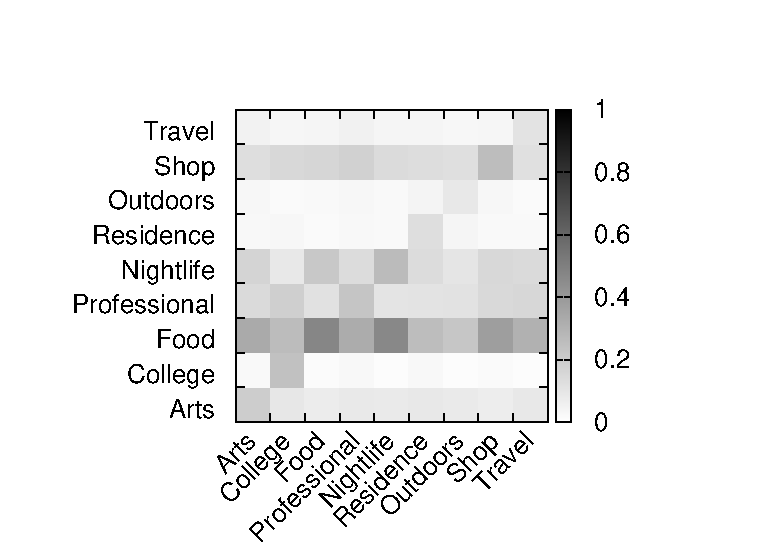
\includegraphics[width=\columnwidth]{plot/ColorMap/Shop_and_Service_and_Professional_and_Other_Places_neighbor_within_100m.eps}
  \end{minipage}\\%[-10pt]

  \begin{minipage}[t]{.4\linewidth}
    \caption{No other POIs within 100m}
    \label{fig:NoPOI}
  \end{minipage}%
  \hspace{0.3cm}
  \begin{minipage}[t]{.55\linewidth}
    %\caption{Shop \& Service's and Professional \& Other Places 's neighbor within 100m}
    \caption{Different categories'(xtics) category distribution(ytics) within 100m}
    \label{fig:ShopProf}
  \end{minipage}%
\end{figure}

\subsection{ The Nearest K POIs}
%\begin{figure}[ht]
%\begin{minipage}[ht]{0.5\linewidth}
%\centering
%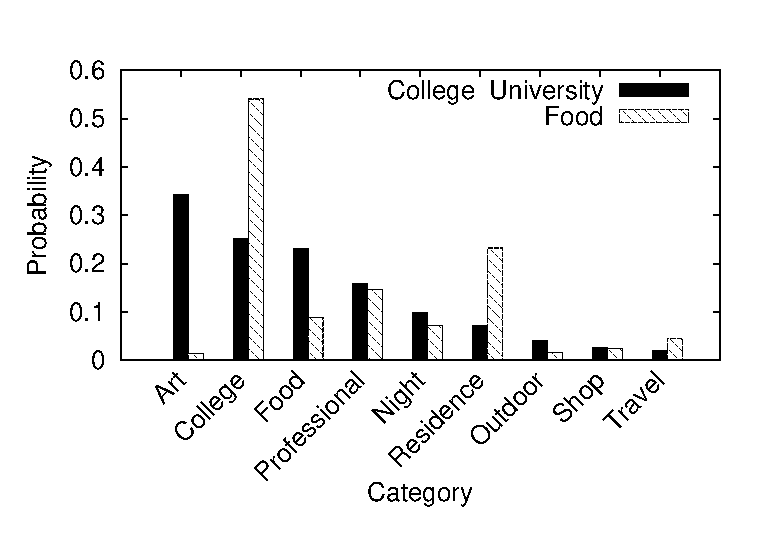
\includegraphics[width=\columnwidth]{plot/Food_and_College_1-Nearest_POI_category_distribution.eps}
%\caption{Food's \& College's 1-Nearest POI category distribution}
%\label{fig:foodcollege}
%\end{minipage}
%\begin{minipage}[ht]{0.5\linewidth}
%\centering
%\includegraphics[width=\columnwidth]{plot/F1_measure_using_N_5_feature.eps}
%\caption{F1 measure using N\_5 feature}
%\label{fig:F1N5}
%\end{minipage}
%\end{figure}


Apart from neighborhood functionality, we find the nearest $k$ POIs'
category as another feature to compensate the NB\_m feature.
It is because the NB\_m feature represents the general
functionality in a big area, but there are often some
concentrations on specific spots. As showed in Figure \ref{fig:foodcollege},
``Food'' and ``College \& University'' show typical intention
aggregating on some spots. For ``College \& University'', no matter
they locate in urban or suburban, the college buildings are definitely
close to each other. And for ``Food'', we can see the trend very often
in our life: there might be a street of local snack, or a part of
business zone full of restaurants. Besides that, other than similar POIs
aggregating together, some categories instinctively near together.
For example, ``Nightlife Spot'' are often mixed with ``Food'',
which is another typical characteristic for both ``Nightlife Spot'' and ``Food''.

It seems that the nearest $k$ POIs feature is a part of POI's neighborhood feature.
However, focusing on the nearest POIs gives extra information on the particular spot the POI is on.
For example, although the neighborhood mainly consists of office buildings,
if the target POI lies in a part of the region that is full of restaurants,
it is more possible that the POI belongs to ``Food''.
In other words, POI's neighborhood is considering a neighborhood based on
the absolute distance, which not only represents the neighborhood's attribute,
but also tells how bustling within the region.
The nearest $k$ POIs feature is a relative neighborhood which considers
only the nearest $k$ POIs, no matter they are far away from each other
or very close to each other. In fact, the two kinds of feature do show
big difference in experiment and we cannot replace one to another.

We use N\_k to abbreviate the nearest k POIs' category distribution.
The N\_k feature is defined as: for a POI i, the category distribution of nearest $k$ POIs within 1km to $i$.

%We further test the influence of selection of k on the result setting $k=1,5,10,20$. According to our experiment, having larger k won't change result very much, we show ``Food'' and ``Nightlife Spot'' as example in Figure \ref{fig:F1NKFoodNight}. However, as we will discuss more in Chapter \ref{Experiment}, since different m in NB\_m will differ very much in result and different m combining different k in N\_k feature will also results in different result, accordingly different k will be needed in final feature construction for different categories.


%{\centering
%\begin{minipage}[ht]{0.5\linewidth}
%\centering
%\includegraphics[width=\columnwidth]{plot/F1_measure_using_N_K_feature_on_Food_and_Nightlife_Spot.eps}
%\captionof{figure}{F1 measure using N\_K feature on Food and Nightlife Spot with different K}
%\label{fig:F1NKFoodNight}
%\end{minipage}
%\begin{minipage}{0.49\linewidth}
%  \centering
%  \small
%  \begin{tabular}{ll}
%
%  \hline\noalign{\smallskip}
%  Category & Distance(m)  \\
%  \noalign{\smallskip}\hline\noalign{\smallskip}
%  Professional \& Other Places  &    210.851 \\
%  Nightlife Spot  &   227.3833 \\
%  Shop \& Service  &   227.5524 \\
%  Arts \& Entertainment  &   230.5648 \\
%  Food  &   237.8074 \\
%  College \& University  &    275.849 \\
%  Residence  &   308.1981 \\
%  \noalign{\smallskip}\hline
%  \end{tabular}
%  \captionof{table}{Different categories' average distance to nearest ``Travel and Transport''}
%  \label{tab:DisToTravel}
%\end{minipage}
%
%}



\begin{figure}[ht]
\centering
%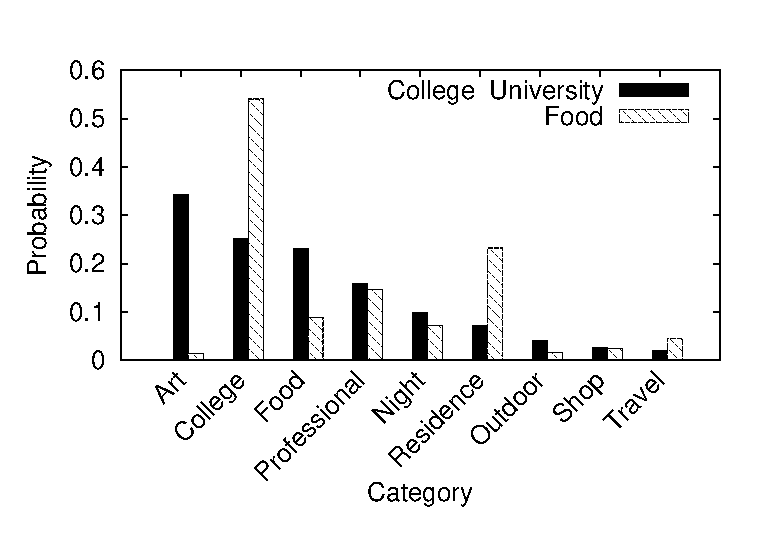
\includegraphics[width=0.7\columnwidth]{plot/Food_and_College_1-Nearest_POI_category_distribution.eps}
\includegraphics[width=0.8\columnwidth]{plot/ColorMap/Food_and_College_1-Nearest_POI_category_distribution.eps}
\caption{Food's \& College's 1-Nearest POI category distribution}
\label{fig:foodcollege}
\end{figure}

\subsection{ Distance to Category}
\label{sec:lcd}
The NB\_m and N\_k feature are insufficient to identify the category for a
POI in some cases. For example, if a POI is located close to a lot of restaurants,
then the POI is supposed to be in category ``Food'' according to the NB\_m and N\_k features.
However, if the POI is far from ``Shop \& Services''
and ``Art \& Entertainments'', then the
POI is probably not a restaurant but a residence.
Due to this fact, we also examine the influence of category
distance, which is the distance from the target POI to
the nearest POI in each category.
%With the NB\_m feature and N\_k feature above, we have a good representation
%for the POIs near the target POI. However, we haven't considered those POIs
%which are not in $m$ meters in NB\_m, and not in the top $k$ list in N\_k.
%There's also a reason why those POIs are, in some sense, far away from the target POI.
%So in order to extract valid information from the POIs that are not near,
%we utilize the feature that shows the distance to the nearest POI in different
%categories, and it exhibits more characteristics. For example, from above
%features including NB\_m and N\_k, a POI shows that it is located close to
%``Food'', based on these, the POI belonging to ``Food'' is a reasonable
%prediction. However, if distance to categories feature tell us more that the
%POI is far from ``Shop \& Services'' and ``Art \& Entertainments'', then the
%probability of the POI belonging to ``Residence'' also rise up.
%We found some interesting facts about category distance.
Specifically, we first examine different categories' average distance
to nearest ``Travel and Transport'' to see which categories are often
near transportation. We show the distances in Table \ref{tab:DisToTravel},
and we find that ``Professional \& Other Places'' is the nearest to transportation,
which is quite reasonable since otherwise the cooperation need to run regular bus for its employees.

\begin{table}[ht]
\centering
%\small
% table caption is above the table
\caption{Different categories' average distance to nearest ��Travel and Transport��}
\label{tab:DisToTravel}       % Give a unique label
% For LaTeX tables use
\begin{tabular}{llll}
\hline\noalign{\smallskip}
Category & Distance(m) &Category & Distance(m) \\
\noalign{\smallskip}\hline\noalign{\smallskip}
Professional \& Other Places  &    \textbf{210.851} &   College \& University  &    275.849   \\
Nightlife Spot  &   227.3833 &Residence  &   308.1981 \\
Shop \& Service  &   227.5524 &Travel \& Transport  & 9788.035\\
Arts \& Entertainment  &   230.5648 &  Outdoors \& Recreation & 12272.19\\
 Food  &   237.8074 & & \\
\noalign{\smallskip}\hline
\end{tabular}
\end{table}

Then, we examine the distance of each category to all other categories in Figure \ref{fig:LogCD}.
From the figure, we observe that ``Outdoor \& Recreation'' is far from all categories,
while ``Food'' is near to all.
This fact gets along with our analysis in Figure \ref{fig:NoPOI} that
there's very few POIs near ``Outdoor'', but ``Food'' can be found everywhere.

Formally, we define the category distance feature ($CD$) for a POI $i$ and a category $c$ as:
\begin{equation}
CD_{i,c}= min_{j \in c} distance(i,j).
\end{equation}

The linear definition of category distance is straightforward but not close to
the fact. POIs in 100km from the target POI and those in 200km
have not much difference for identifying the target POI's category because
both of them are too \emph{far}. In contrast, the classifier should be sensitive
to the difference between two short distances. Therefore, we propose two
variations to $CD$, i.e., $LCD1, LCD2$ as follows:
\begin{align}
LCD1_{i,c} &= \log{(1+CD_{i,c})},\\
LCD2_{i,c} &= \log{(1+\log{(1+CD_{i,c})})}.
\end{align}



%According to our experiment, directly using $CD$ as features in classification is not effective, and a reasonable process is to take log operation, therefore we further define $LCD1, LCD2$ as, for each POI $i$,
%\begin{align}
%LCD1_i &= Log(1+CD_i)\\
%LCD2_i &= Log(1+ Log(1+CD_i))
%\end{align}


%\begin{figure}
%\begin{minipage}[ht]{0.5\linewidth}
%\centering
%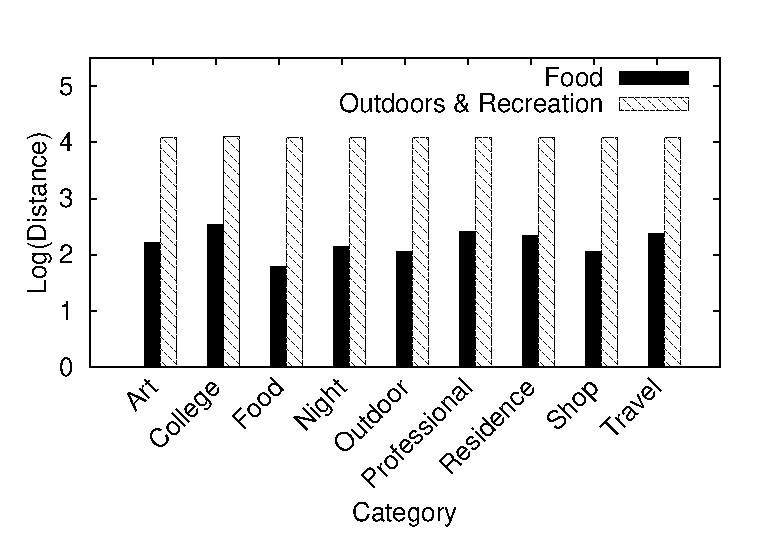
\includegraphics[width=\columnwidth]{plot/LogAvgCD.eps}
%\caption{Log(Avg(Category Distance))}
%\label{fig:LogCD}
%\end{minipage}
%\begin{minipage}{0.5\linewidth}
%  %\centering
%  %\raggedleft
%  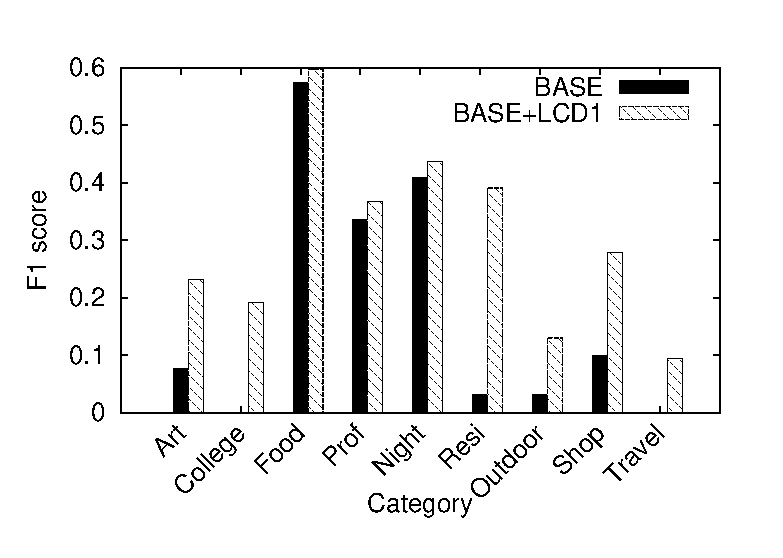
\includegraphics[width=\columnwidth]{plot/F1_measure_using_LCD1_feature.eps}
%  \caption{F1 measure using LCD1 feature}
%  \label{fig:F1LogCD}
%\end{minipage}
%
%\end{figure}

\begin{figure}[ht]
\centering
\includegraphics[width=0.8\columnwidth]{plot/ColorMap/Color_CategoryDis.eps}
%\caption{Log(Avg(Category Distance))}
\caption{Average Category Distance with log operation, darker indicates a larger distance}
\label{fig:LogCD}
\end{figure}

\subsection{ Region Comparison}


%\begin{figure}[ht]
%\centering
%% Use the relevant command to insert your figure file.
%% For example, with the graphicx package use
%  \epsfig{file=plot/F1_measure_using_RegCom_T_feature.eps,width=0.7\columnwidth}
%% figure caption is below the figure
%\caption{F1 measure using RegCom feature}
%\label{fig:F1RC}       % Give a unique label
%\end{figure}
Region Comparison feature aims at comparing the target POI with other POIs within
the same region on the user behaviors. The motivation is that some categories
may often be ``destinations'' of a user's travel activity, such as ``Art \& Entertainment'',
while some categories may often be on the way to the destination, such as ``Food''.
We assume that the places which are more popular (according to users and check-ins) than other places nearby,
is more probable to be a destination. To make use of the user check-in information,
we consider both the number of check-ins and the number of unique users. We compare
the check-ins and unique users of the target POI to the POIs within a distance of m,
and compute the average difference of check-ins and unique users as the
region comparison feature for the POI. The region comparison feature for total
check-ins (RC\_T\_m(i,c)) and for unique users (RC\_U\_m(i,c)) are computed as follows:
%Thus with such feature, we combine
%the factor from both spatial environment and user behavior. As for user behavior,
%inspired by the previous work, we consider the number of check-ins and unique users.
%Therefore, we compare the target POI's number of total check-ins and unique users
%with the POIs around it, and the region is precisely defined by a radius of m.
%In NB\_m, we apply different m to define neighborhood for different categories,
%likewise, we also build several different Region Comparison features with different m.
%In terms of comparison, we do substraction between the average level of user behavior measures and the target POI's digits. Formally, we define $Region Comparison\_Total Check-in (RC\_T\_m)$ and $Region Comparison\_Unique Users (RC\_U\_m)$ as
\begin{equation}
RC\_T\_m(i,c) = Avg_{j \in c, distance(i,j)<m} \#Checkin(j) - \#Checkin(i) 
\label{eq:rct}
\end{equation}
\begin{equation}
RC\_U\_m(i,c) = Avg_{j \in c, distance(i,j)<m} \#UniqueUser(j) - \#UniqueUser(i)
\label{eq:rcu}
\end{equation}

Figure \ref{fig:RC} shows the average region comparison feature of 
total check-ins for the five categories of POIs.
The score below 0 means that people check in more times at target POI than the POIs near it.
%Checking in a place more than the ones near it is actually saying that people are gathered to the place, or in other word, it is a ``destination'', not a ``by the way''.
Intuitively, ``Art \& Entertainment'' is more of a ``destination'', people come in purpose
to watch a show, or see an exhibition. ``Outdoor \& Recreation'' is more of a ``destination'', too,
since people planned beforehand to have a weekend with children on a beach, or have a routine of
going to fishing spot. ``Food'' is a ``on the way'' category both by intuition and statistics.
People grab something to eat all the time: after a walk or before a movie. Interestingly, we
find that ``Shop \& Service'' shows the character of a ``by the way'', too.
It seems interesting shops are growing in number, and consequently people are attracted into a
shop though not intended. In contrast, nightlife spot's are more of destinations, because they 
are usually the last places people may visit in daily life. 
%it seems bars are getting more popularity and loyalty from customers than shops and food.

%To show the strength of region comparison features, we set m to be 100 for both RC\_T\_m and RC\_U\_m, and test the features on the nine first level categories, the result is shown in Figure \ref{fig:F1RC}. When the features are combining with BASE and m set to be 100, RC\_T\_m and RC\_U\_m show similar strength in classification, however, as we will discuss more on experiment in Chapter \ref{Experiment}, RC\_U\_m appears to be more effective than RC\_T\_m. Overall, they do show improvements but not as powerful as previous ones.
\begin{figure}[ht]
% Use the relevant command to insert your figure file.
% For example, with the graphicx package use
  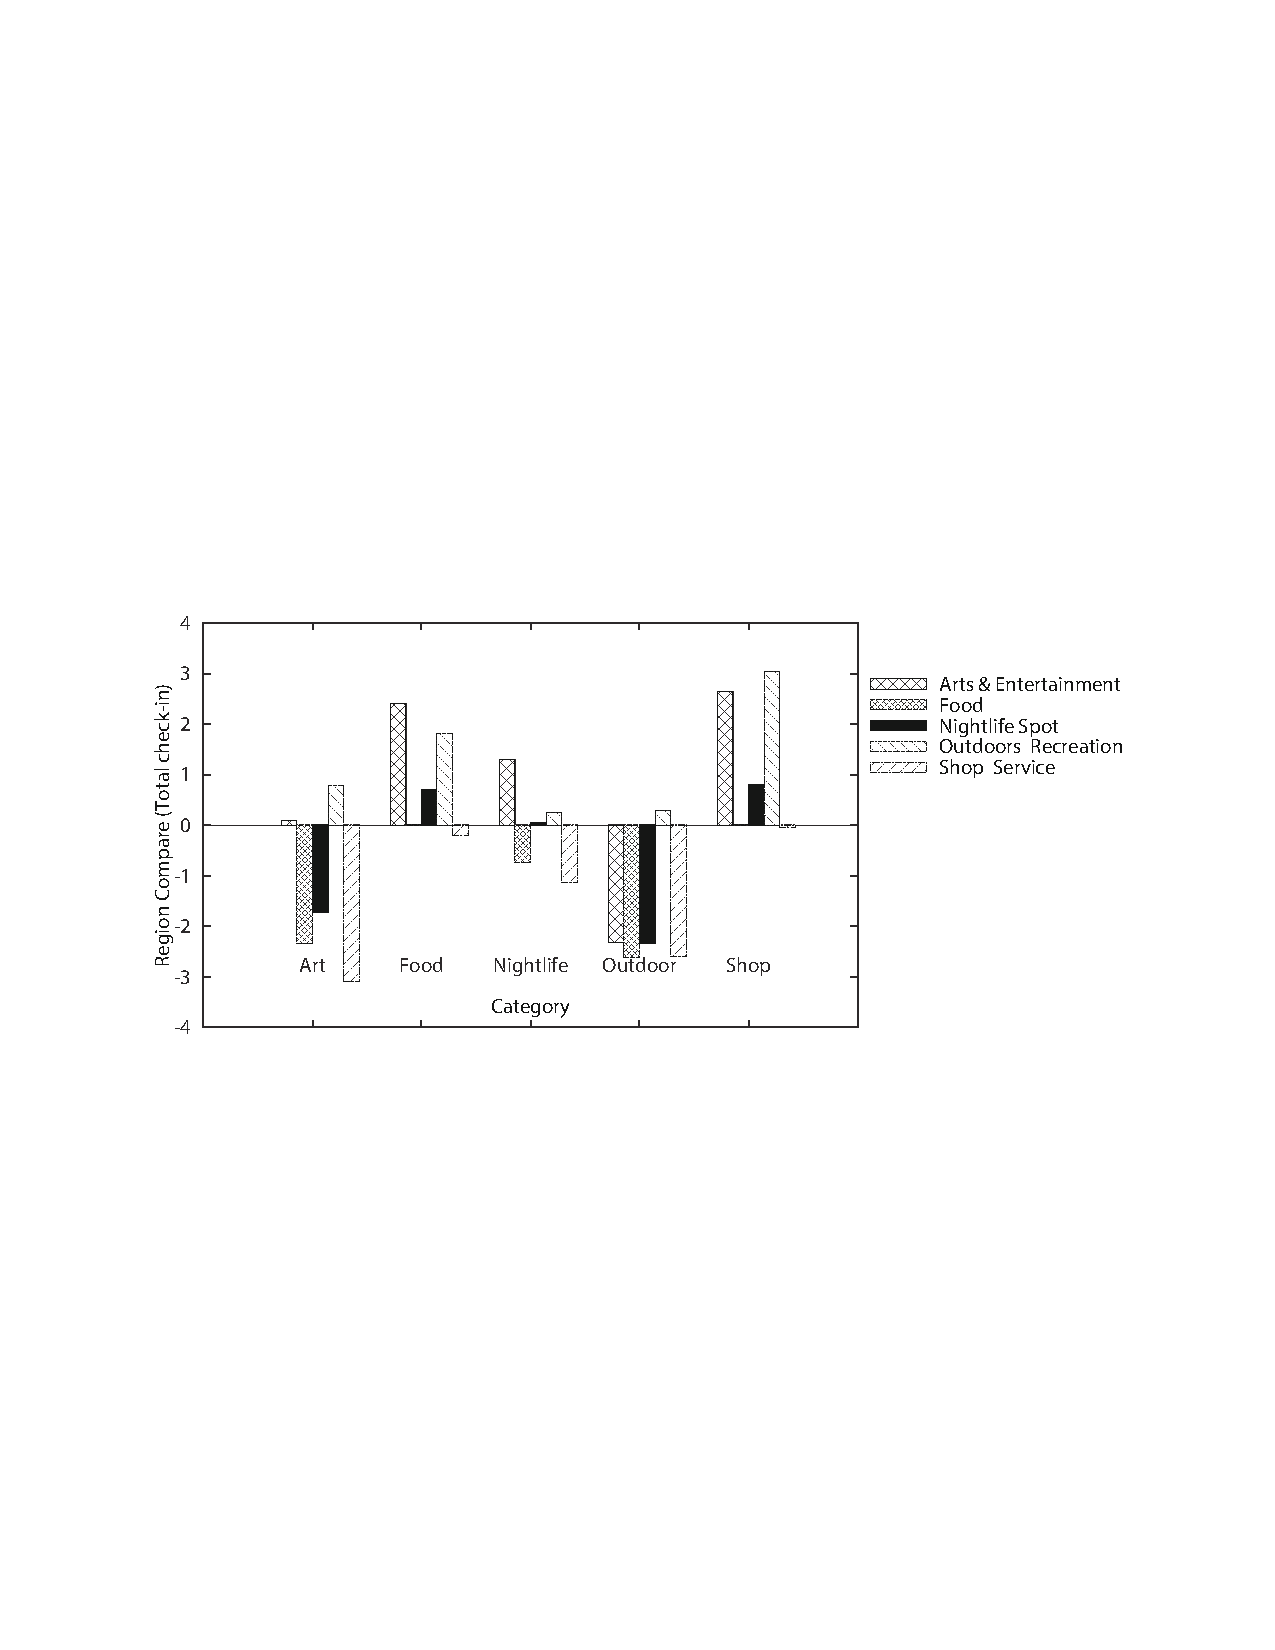
\epsfig{file=plot/RegionCompare.pdf,width=\columnwidth}
% figure caption is below the figure
\caption{Region Compare (Total Check-ins), score below 0 indicates more check-in time than other categories within same region}
\label{fig:RC}       % Give a unique label
\end{figure}

\section{Other Features}
\label{chp:others}
\subsection{NAME Features}
The most direct way to discover the category of a POI is looking at its name.
%Similar with human guessing the category of a POI, the first intuition we get from a POI is its name.
For example, when we see a POI named ``Mouth Restaurant'', we would easily figure out that it belongs to ``Food''.
%Given the fact that words appear in POIs' names are far more less than in vocabulary,
We build the NAME feature in a straightforward way. We break POIs' names into words,
then we collect all the words and filter out those showed up only once in POIs.
Then the remaining words forms a dictionary, and NAME feature for a POI is the
binary representation of the POI's name in the dictionary.

Simple as it is, it is obvious that NAME feature is a powerful feature.
However, there's still cases that name features cannot help but other features work.
For example, when we meet the name ``Charlie's Corner'', it is not so obvious what category
it should belong to by looking at the name. However, it shows good visit time distribution,
as well as good spatial environment character with other ``Food'' near it,
thus we still can classify it to ``Food'', which is the correct label, over other categories.

\subsection{BASE Features}
\label{sec:base}
As discussed above, the statistics of user behavior
features in Ye et al.'s work \cite{yemao} are also effective features for identifying
a POI's category. We also employ these feature in our experiments.
These features include the total number of check-ins, unique visitors,
maximum number of check-ins by a single visitor, distribution of check-in
time in a week and in 24-hour scale. %Such features represent the user behavior very well.



\section{Evaluation Framework}
\label{sec:eval_frameworks}
% \KZ{Are we only evaluating the final version of the two bots from prev section? This is not part of the iterative design process right? This should be made clearer.}
% \MY{normally we provide objective/automatic eva first, followed by human evaluation results. when introducing the metrics and results, follow this order}

This section describes our evaluation framework, covering interactive experiments for ``human-bot'' chats, along with diverse task-specific metrics. Aligned with proposed objectives, this framework can be applied to evaluate the performance of various psychiatrist and patient chatbots.

\subsection{``Human-bot'' Interactive Chat}
The human evaluation measure is widely considered as golden metric for dialog system. In contrast to the approach of using actors/actresses to simulate patients as mentioned in \citet{yao-etal-2022-d4}, our evaluation process involves \textit{actual depression patients} interacting with psychiatrist chatbot and \textit{human psychiatrists} interacting with patient chatbot. 
This approach allows us to evaluate the performance of these two types of chatbots in real-world scenarios.
We introduce our participants as follows:

\paragraph{Depressive individuals} were recruited through online advertisements, resulting in the participation of 14 volunteers aged 18 to 31. The gender distribution was 28.57\% male and 71.43\% female. 

\paragraph{Psychiatrists} were invited through cooperation with hospitals. We invited 9 psychiatrists, two of them are graduate students majoring in psychiatry, and the rest are practicing psychiatrists with rich clinical experience to ensure the professionalism of the evaluation.

\paragraph{Evaluation Procedure}
We adhere to standard human evaluation procedures~\cite{Yue2023Beyond}, where each participant engages with all the chatbots in random order, and rates their performance after a full conversation with each one. Once participants conclude interactions with all chatbots, they are instructed to adjust their original ratings to ensure that each chatbot receives different scores in the same metric. 

\subsection{Evaluation Metrics}
\label{sec:eval_metric}
When designing evaluation metrics, our goal is to ensure that each objective is accompanied by appropriate metrics for accurate measurement.  We employ both rating and computational metrics for evaluation. \textbf{Rating metrics} are scored by humans after interactive conversations with the chatbot, while \textbf{computational metrics} can be calculated based on the dialog history.  
We divide the computational metrics of both kind of chatbots into two types: \textit{function} and \textit{style}. The overview of these metrics and their relations to objectives can be found in \figref{fig:all_metric}.
% \MY{Clearer now, but still mixing function and style - which objectives and metrics are function-related and which are style?}.
% NEWCOMMENT: 这里这样分类之后,在图中也要把两类指标区分出来,可以在objective那一列上做区分
\begin{figure}[th]
	\centering
	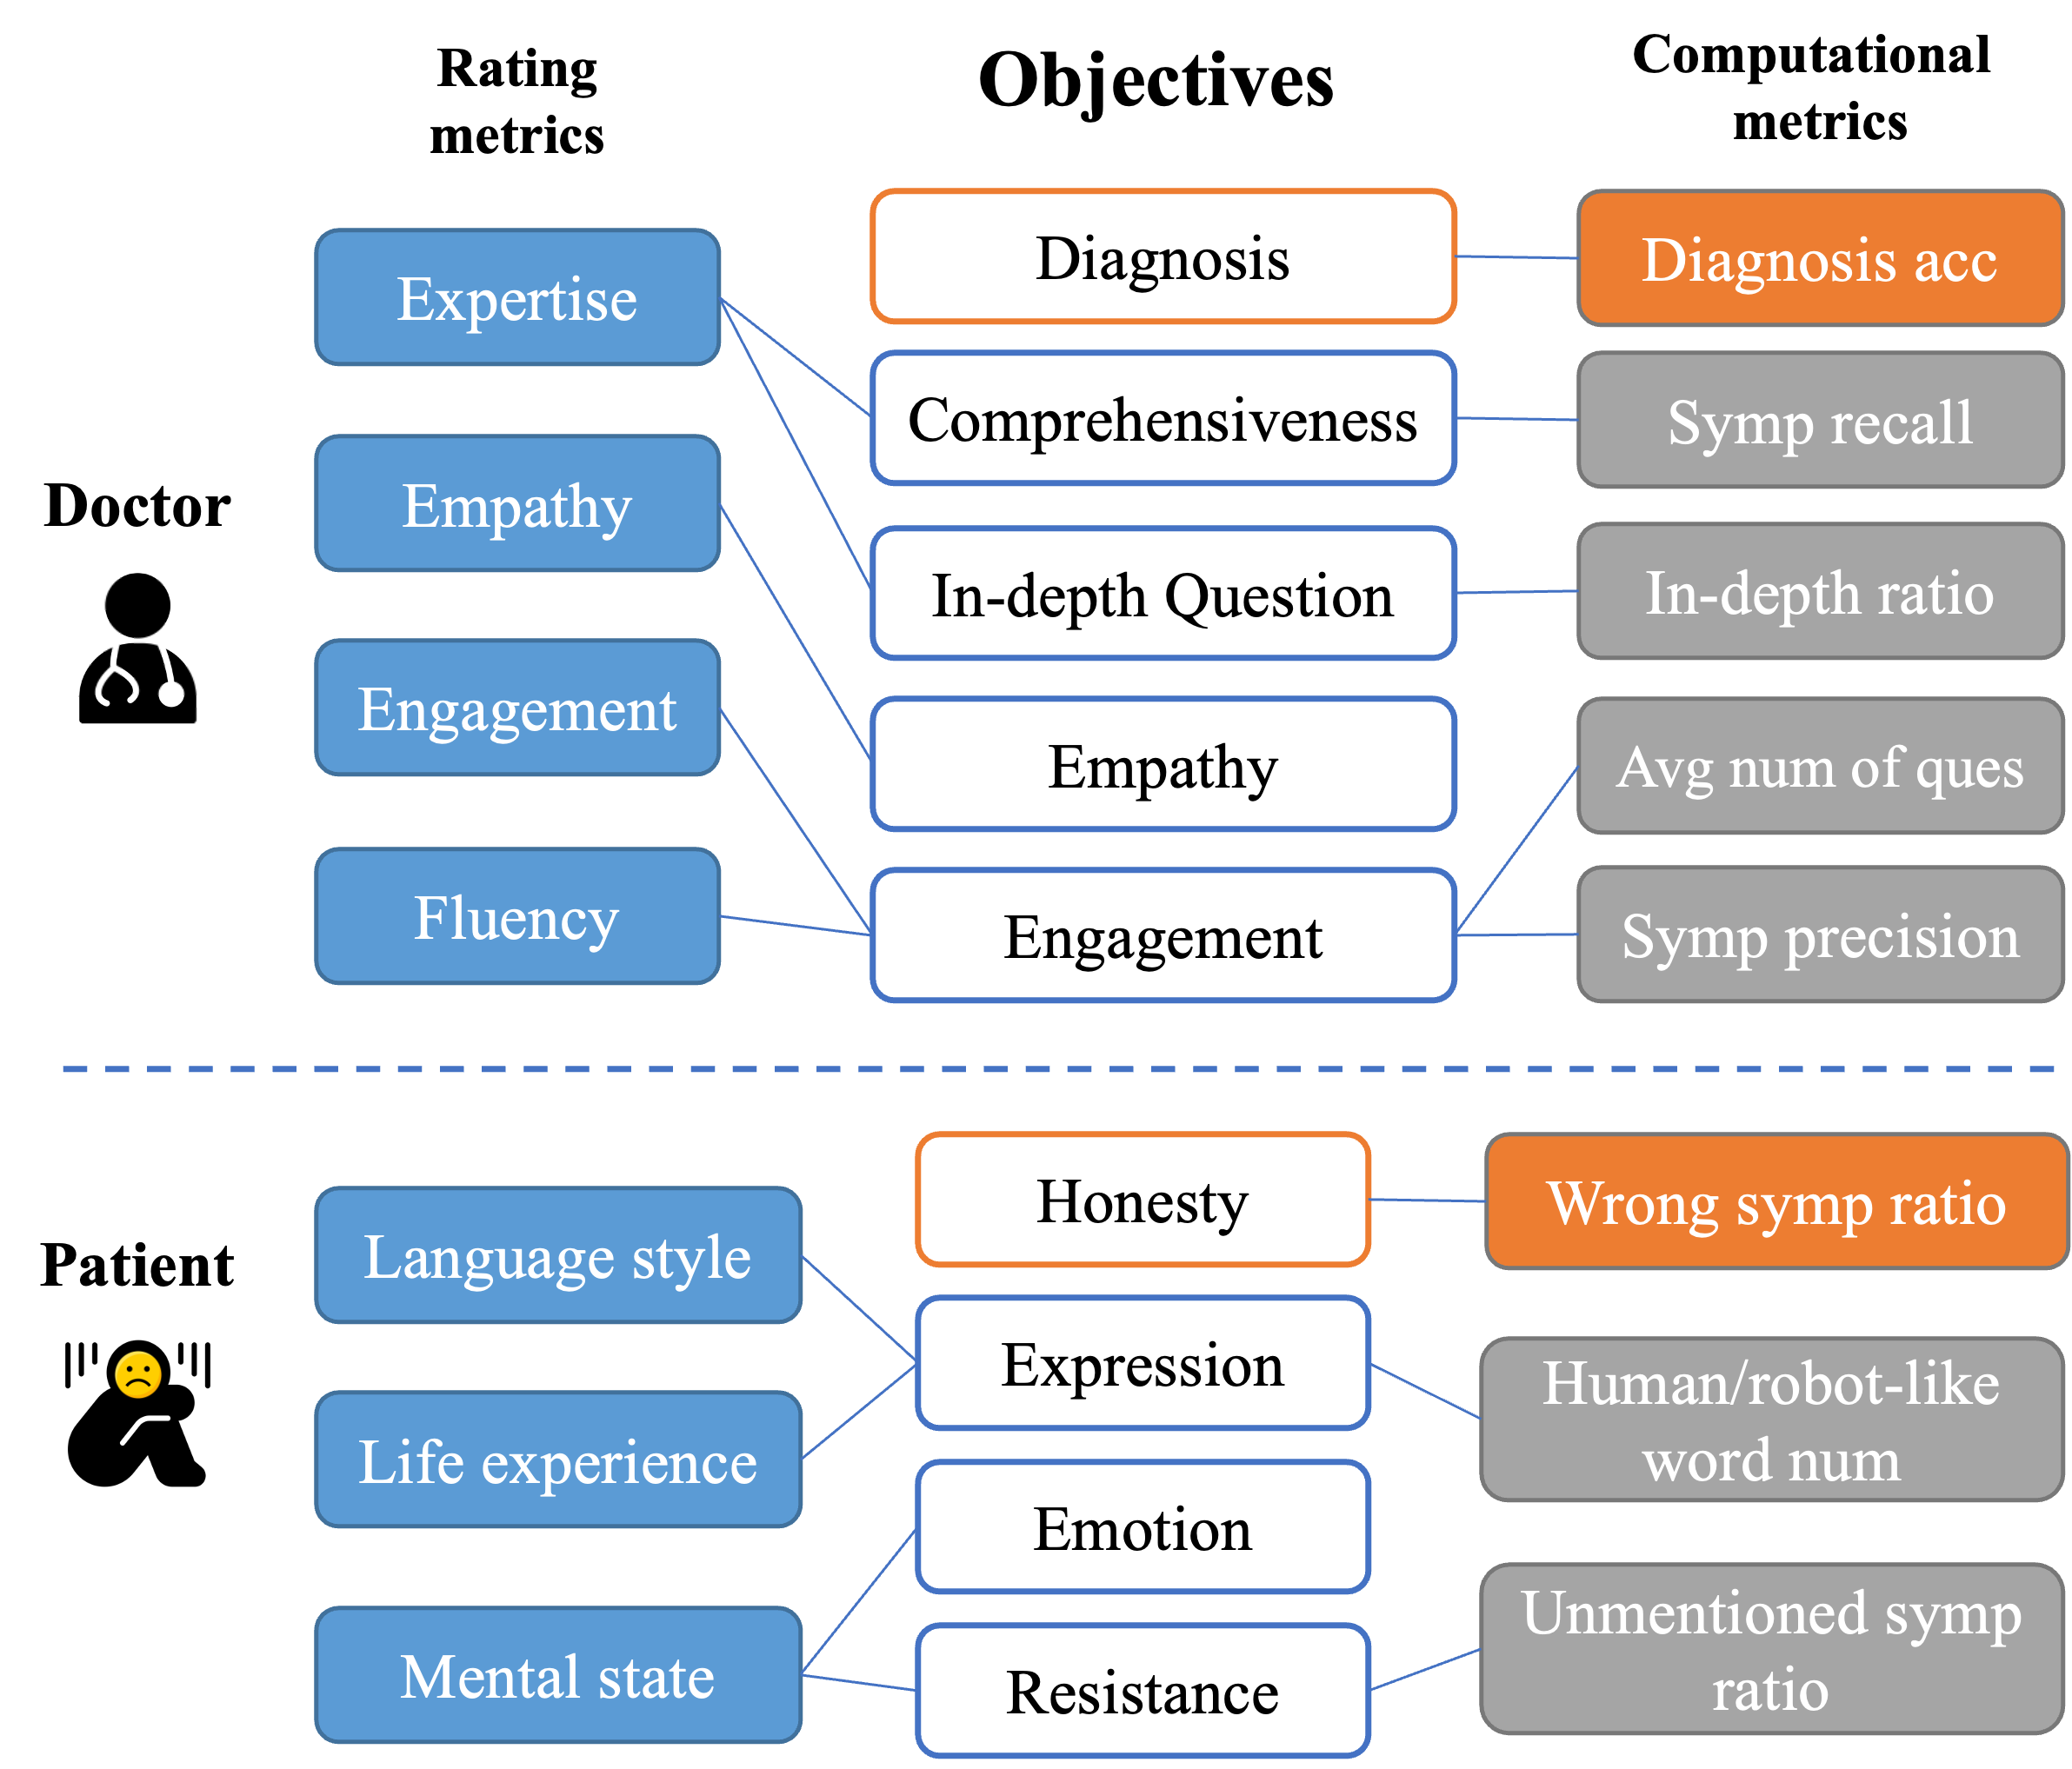
\includegraphics[width=\linewidth]{Figures/metrics_new.png}
	\caption{The correspondence between evaluation metrics and objectives. \textbf{\textit{Function}} metrics are orange, and \textbf{\textit{style}} metrics are gray.}
	\label{fig:all_metric}
\end{figure}

\subsubsection{Metrics for Psychiatrist Chatbot}
\paragraph{Rating Metrics} 
We mainly focus on the user experience for rating metrics of psychiatrist chatbot, as shown in Table \ref{tab:human_eval_doctor}. This emphasis stems from the fact that, in most cases, patients lack specialized knowledge in psychiatry, making it challenging for them to precisely assess a doctor's professional skills.
% In most cases, patients do not have specialized knowledge in psychiatry, making it difficult for them to assess a doctor's professional skills precisely. Therefore, we focus mainly on the user experience for rating metrics of psychiatrist chatbot, as shown in Table \ref{tab:human_eval_doctor}.
\begin{table}[h]
    \centering
    \footnotesize
    \begin{tabular}{m{0.18\columnwidth}|m{0.7\columnwidth}}
    \hline
    Metrics & Explanation \\
    \hline
    Fluency & The chatbot does not repeat previously asked questions and can smoothly switch between different topics. \\
    \hline
    Empathy & The chatbot can understand and comfort you properly. \\
    \hline
    Expertise & The chatbot behaves like a real doctor, making you believe in its professionalism. \\
    \hline
    Engagement & The chatbot can maintain your attention and make you want to continue talking to it. \\
    \hline
    \end{tabular}
    \caption{Rating metrics of psychiatrist chatbot.}
    \label{tab:human_eval_doctor}
\end{table}
\paragraph{Computational Metrics}
Different from rating metrics, we mainly measure the expertise of the psychiatrist chatbot using computational metrics based on dialog history.
The \textit{functional} requirements for psychiatrist chatbot is to provide an accurate diagnosis, so the corresponding metric is \uline{``diagnosis accuracy''}. 
The \textit{style} part concerns the psychiatrist chatbot's professional skills. We use \uline{``symptom recall''} to evaluate the chatbot's ability to comprehensively gather the patient's symptom-related information, and use \uline{``in-depth ratio''} to assess the ability to ask in-depth questions for deeper understanding. 
To ensure a better user experience, we calculate the \uline{``average number of questions''} asked in a single interaction to discourage the chatbot from overwhelming patients with excessive queries. Furthermore, we employ the metric of \uline{``symptom precision''} to penalize the chatbot's mechanistic behavior of asking all potential questions, irrespective of the user's responses\footnote{A detailed explanation of these computational metrics can be found in Appendix \ref{apd:eval}.\label{footnote:comp_metric}}. 

\subsubsection{Metrics for Patient Chatbot}
\paragraph{Rating Metrics}
There is no standard to measure whether a patient is ``good'' enough. Thus, when chatting with patient chatbots, doctors can only assess whether their style of expression and manner of communication resemble real patients enough and whether they can describe their symptoms in a reasonable way, so the main metrics for rating are \textbf{Resemblance} and \textbf{Rationality}.
We further divide the Resemblance metric into three aspects in Table \ref{tab:human_eval_patient}, according to the objectives in Section \ref{sec:objectives}.

\begin{table}[h]
    \centering
    \footnotesize
    \begin{tabular}{m{0.18\columnwidth}|m{0.65\columnwidth}}
    \hline
    Metrics & Explanation \\
    \hline
    Mental State & The chatbot is in depressed state, such as be in low mood, reluctance to communicate, scattered thoughts, etc.\\
    \hline
    Life Experience & The description of symptoms is related to daily life and personal experiences.\\
    \hline
    Language Style & Use colloquial and natural expressions when describing symptoms.\\
    \hline
    \end{tabular}
    \caption{Three aspects of the ``Resemblance'' metric.}
    \label{tab:human_eval_patient}
\end{table}
\paragraph{Computational Metrics}
The \textit{functional} requirement of patient chatbot is ``honesty'', and we can calculate \uline{``wrong symptom ratio''} by comparing the patient's symptom list with the symptoms it reported to assess this aspect. 

Then, we evaluate the patient chatbots' \textit{style} using some linguistic features, like \uline{``Human/robot-like word ratio''}, to find out whether their language is colloquial with limited usage of professional terminology. We also use \uline{``unmentioned symptom ratio''} to measure the resistance level of chatbots\textsuperscript{\ref{footnote:comp_metric}}. 

% \subsection{Human Evaluation}
% The human evaluation measure is widely considered as golden metric for dialog system. In contrast to the approach of using actors/actresses to simulate patients as mentioned in \citet{yao-etal-2022-d4}, our human evaluation process involves actual depression patients, enabling us to assess the performance of chatbots in real-world scenarios.

% Depression patients were recruited through online advertisements, resulting in the participation of 14 volunteers aged 18 to 31. The gender distribution was 28.57\% male and 71.43\% female. 

% First, to assess the severity of participants' depression, they were asked to complete the Beck Depression Inventory~\cite{beck1996beck}, yielding a score ranging from 0 to 63. Notably, we have a balanced distribution of subjects across various depression levels: $healthy_{(0-13)}$, $mild_{(14-19)}$, $moderate_{(20-28)}$ and $severe_{(29-63)}$ according to the Beck Depression Score\footnote{Refer to Table \ref{tab:distribution_seve} in Appendix \ref{apd:eval} for the distribution details.}.
% We adhere to standard human evaluation procedures~\cite{Yue2023Beyond}, where each participant engages with all the psychiatrist chatbots in random order, and rates their performance after a full conversation with each one. Once participants conclude interactions with all chatbots, they are instructed to adjust their original ratings to ensure that each chatbot receives different scores in the same metric. 

% We carefully design human evaluation metrics \KZ{sentence incomplete.}

\subsection{Computation and Annotation}
% A detailed explanation of the automatic metrics for the doctor and patient chatbot can be found in Appendix \ref{apd:eval}. \MY{This sentence can put in footnote, a bit distracted to start a new subsection with reference to appendix. Say things like "We establish comprehensive and quantitative metrics like xx, xx, and xxx, each covering xx xx aspects. footnote, details can be found in ..."}

To obtain the ground truth score of the metrics ``diagnosis accuracy'', each participant engaging with our psychiatrist chatbot is invited to complete the Beck Depression Inventory~\cite{beck1996beck} to evaluate the severity of their depression.

In addition, to calculate some of these metrics, we need to annotate the dialog history. This involves identifying the relevant symptom in the doctor's question, determining whether the patient truly experiencing a certain symptom, and so on, which is described in Appendix \ref{apd:annotation}.

% First, to assess the severity of participants' depression, they were asked to complete the Beck Depression Inventory~\cite{beck1996beck}, yielding a score ranging from 0 to 63. Notably, we have a balanced distribution of subjects across various depression levels: $healthy_{(0-13)}$, $mild_{(14-19)}$, $moderate_{(20-28)}$ and $severe_{(29-63)}$ according to the Beck Depression Score\footnote{Refer to Table \ref{tab:distribution_seve} in Appendix \ref{apd:eval} for the distribution details.}.

% Due to the inadequacy of dialogue history data for training multiple classification models, we employ ChatGPT to automatically label each sentence in the dialogue history, leveraging its impressive annotation capabilities~\cite{Gilardi2023ChatGPTOC}. Subsequently, three annotators thoroughly review and rectify the results to ensure the quality of the annotation.
% To assess the performance of dialogue systems, it is crucial to employ both human evaluation and automatic metrics, especially in mental health domain. Since there is little previous work on how to evaluate simulated psychiatrists and patients, we design several task-specific metrics and interactive experiments for human evaluation. 

% \subsection{Human Evaluation Participants}
% % We first implemented a website to host our chatbots, making it easier for participants to interact with them and rate their performance. The details of the website can be found in Appendix \ref{sec:chatInterface}. 
% %\subsubsection{Participants}
% In contrast to the approach of using actors/actresses to simulate patients as mentioned in \citet{yao-etal-2022-d4}, our evaluation process involves actual depression patients and psychiatrists, enabling us to assess the performance of chatbots in real-world scenarios.

% Depression patients are recruited through online advertisements.
% A total of 14 volunteers completed the entire process. Their age ranges from 18 to 31, while 4 of them are male, while the rest of female. 
% To assess the severity of their depression, patients are asked to complete the Beck Depression Inventory~\cite{beck1996beck}. Notably, we have a balanced distribution of healthy, mild, moderate and severe depression subjects which distribution is presented in Table \ref{tab:distribution_seve} in Appendix \ref{apd:eval}.
% % \KZ{If the severity is ``none'', this patient is considered healthy?}

% We invited 9 psychiatrists who are not involved in the prompt design, through cooperation with hospitals. Two of them are graduate students majoring in psychiatry, and the rest are practicing psychiatrists with rich clinical experience to ensure the professionalism of the evaluation.
%!TEX root = paper.tex

\section{Related Work}
\label{sec:related}

MLlib, Mahout \cite{mahout}, and MADLib \cite{madlib} are machine learning \emph{libraries} on top of distributed computing platforms and relational engines.
All of them provide many standard machine learning models such as LDA and SVM.
However, when a domain user, say, a machine learning researcher, 
is devising and testing her customized models with her big data, 
those libraries cannot help.

MATLAB and R have been the most popular systems for implementing inference algorithms.
They, however, can hardly scale up when faced with increasing amount of data
because they mostly work on a single machine and thus cannot easily scale out.
It is possible to first transform a large dataset into a smaller one
using MapReduce or Spark and then load the data to MATLAB or R to perform inference %on the smaller ones in
in some scenarios. But this approach involves multiple systems, which is hard to
develop code for and inefficient because of the data movement.
SystemML \cite{systemml} provides a similar interface for implementing inference
algorithms and transforms them to Hadoop MapReduce. It can scale out to large
clusters but coding on such a system still requires extensive knowledge in
statistical inference for end-user. 

In contrast to the systems above, MLBase \cite{mlbase} targets end-users who are not
machine learning experts. It exposes a declarative language interface and
provides a cost-based optimizer that selects the best algorithm and
parameters. It also provides MLI \cite{mli}, a set of APIs for customizing algorithms on
Spark. However, MLBase mainly supports frequentist approach, such as SVM,
and logistic regression. It does not deal with general Bayesian inference. 

There are a number of probabilistic programming frameworks other than
Infer.NET \cite{InferNET14}.  For example, Church \cite{GMR+08} is a
probabilistic programming language based on the functional programming
language Scheme.  Church programs are interpreted rather than compiled.
Random draws from a basic distribution and queries about the execution trace
are two additional type of expressions. A Church expression defines a
generative model. Queries of a Church expression can be conditioned on any
valid Church expressions. Nested queries and recursive functions are also
supported by Church. Church supports stochastic-memoizer which can be used to
express nonparametric models.  Despite the expressive power of Church, it
cannot scale for large dataset and models.  Figaro is a probabilistic
programming language implemented as a library in Scala \cite{Figaro}.  It is
similar to Infer.NET in the way of defining models and performing inferences
but put more emphasis to object-orientation. Models are defined by composing
instances of Model classes defined in the Figaro library.  Infer.NET is a
probabilistic programming framework in C\# for Bayesian Inference. A rich set
of variables are available for model definition. Models are converted to a
factor graph on which efficient built-in inference algorithms can be applied.
Infer.NET is the best optimized probabilistic programming frameworks so far.
Unfortunately, all existing probabilistic programming frameworks including
Infer.NET cannot scale out on to a distributed platform.

To the best of our knowledge, InferSpark is the only framework that can
efficiently carry out large-scale Bayesian inference through probabilistic
programming on a distributed in-memory computing platform. It targets
end-users who are not expert in Bayesian inference or distributed computing.
The inference implementation can scale out to a large cluster and scale up to
large datasets.

%
%Our proposed probabilistic programming language is also an extension to the existing language Scala, but differs from the way that Infer .NET and Figaro define models that we add additional language constructs to Scala rather than implement a library. It typically enables a cleaner syntax. 







%\item Other inference algorithms for Bayesian Networks.



\cut{%%%%%%%%%%%%%%
The Apache Hadoop library \cite{hadoop} is a distributed data storage and processing framework. Its distributed file system HDFS support the storage of large data. MapReduce is the programming model for distributed parallel processing of the large data. It is composed of two key operations map and reduce. Map operation transforms and filters the data on different nodes in parallel while reduce operations combines the results from map operation to produce results grouped by keys. In our proposal of PP, data can be distribted on a HDFS.

Spark is another distributed data processing framework that provides MapReduce operations. It differs from Hadoop in that it does not write the intermediate results to temporary storage. Instead, it caches the results in memory as resilient distributed dataset \cite{Zaharia:2012:RDD:2228298.2228301}. It can greatly speed up the processing. 

The Spark built-in machine learning library MLlib \cite{mllib} provides a variety of standard statistical inference algorithms including classification, regression, clustering, collaborative filtering and dimensionality reduction. The algorithms leverage the Spark infrastructure so that large-scale data can be processed efficiently. The algorithms are applicable when the standard models fit the data well. Users have to directly develop their own algorithms using Spark or GraphX API when a customized model has to be used. Our integration of PP with Spark can greatly reduce the amount of work to implement a new model.

GraphX \cite{Xin:2013:GRD:2484425.2484427} is Spark's built-in graph parallel computation API. User can view graphs as normal RDDs of vertices and edges and perform normal map reduce operations on them or perform graph operations like compute subgraph, reversing edges, join vertices. The Pregel operator in GraphX is used to express iterative algorithms. In each step, vertices aggregates messages along the inbound edges from previous step, compute its new value and sends messages along outbound edges in parallel. It terminates when no message is sent during a step. Our PP will be built on GraphX since it is natural to represent the factor graph in GraphX and leverage the parallel graph computing to implement message-passing style inference algorithms.

\KZ{Reduce the discussion of the following PP languages a bit. Focus on
their big-data handling capabilities, or the lack of which.}

Many recent probabilistic programming languages are implemented by extending existing conventional programming languages such as Scheme, C\#, Scala and etc.
We examine three probabilistic programming languages Church \cite{GMR+08}, Infer .NET \cite{InferNET14} and Figaro \cite{pfeffer2009figaro}.

Church is a probabilistic programming language based on the functional programming language Scheme. Random draws from a basic distribution and queries about the execution trace are two additional type of expressions. A church expression defines a generative model. Queries of a church expression can be conditioned on any valid church expressions. Nested queries and recursive functions are also supported by Church. Church supports stochastic-memoizer which can be used to express nonparametric models. Thus a wide range of probabilistic models can be concisely expressed in Church. Inference in Church is implemented by rejection sampling and Metropolis-Hastings sampling algorithms. Despite the expressive power of Church, it cannot scale up to large dataset and models. 

Our approach differs from Church in that our program is compiled rather than interpreted. Compiled program is usually more efficient than interpreted ones. We can also leverage the distributed parallel processing to scale up to large dataset and models.

Infer .NET is a probabilistic programming framework in C\# for Bayesian Inference. A rich set of variables are available for model definition. Models are converted to a factor graph on which efficient built-in inference algorithms can be applied. The algorithms include expectation propagation, variational message passing, block Gibbs sampling. Infer .NET addresses the scalability by shared variables, as discussed in Section \ref{sec:intro}.
%% ?? not sure about how the shared variable is implemented

Figaro is a probabilistic programming language implemented as a library in Scala. It is similar to Infer .NET in the way of defining models and performing inferences but put more emphasis to object-orientation. Models are defined by composing instances of Model classes defined in the Figaro library.

Our proposed probabilistic programming language is also an extension to the existing language Scala, but differs from the way that Infer .NET and Figaro define models that we add additional language constructs to Scala rather than implement a library. It typically enables a cleaner syntax. 

}%%%%%%%%%%%%%%%%

\section{Conclusion}

In this paper, we incorporated the idea of Cookie Theft picture description task into the evaluation of the high-level cognitive abilities of LVLMs and designed a novel evaluation benchmark called CogBench.
% Images in CogBench are of high quality and require more cognitive reasonings to understand, which makes it different from existing image datasets.
The images in CogBench are of high quality and demand more complex cognitive reasoning for interpretation, setting it apart from existing image datasets.
% It consists of a image description task and a VQA task.
Experiments show that there is still a large gap between the cognitive abilities of LVLMs and human beings, indicating CogBench is a challenging benchmark.

% In the future


%{\def\chapter*#1{}
%\clearpage
%\begin{center}\fontsize{14pt}{14pt}\selectfont\bf REFERENCE\end{center}
%\begin{spacing}{1.5}
%\fontsize{12pt}{12pt}\selectfont
%\setcitestyle{numbers}
\bibliography{reference/gcc}
%\end{spacing}}

%{\def\chapter*#1{}
%\clearpage
%\begin{center}\fontsize{14pt}{14pt}\selectfont\bf Acknowledgements\end{center}
%\section{Acknowledgments}

This work is kindly supported by ...

% Identification of funding sources and other support, and thanks to
% individuals and groups that assisted in the research and the
% preparation of the work should be included in an acknowledgment
% section, which is placed just before the reference section in your
% document.

% This section has a special environment:
% \begin{verbatim}
%   \begin{acks}
%   ...
%   \end{acks}
% \end{verbatim}
% so that the information contained therein can be more easily collected
% during the article metadata extraction phase, and to ensure
% consistency in the spelling of the section heading.

% Authors should not prepare this section as a numbered or unnumbered {\verb|\section|}; please use the ``{\verb|acks|}'' environment.}

\end{document}
